% THIS DOCUMENT IS FOLLOWS THE VOLERE TEMPLATE BY Suzanne Robertson and James Robertson
% ONLY THE SECTION HEADINGS ARE PROVIDED
%
% Initial draft from https://github.com/Dieblich/volere
%
% Risks are removed because they are covered by the Hazard Analysis
\documentclass[12pt]{article}

\usepackage{booktabs}
\usepackage{tabularx}
\usepackage{hyperref}
\usepackage{float}
\usepackage{graphicx}
\usepackage{longtable}
\usepackage{enumerate}
\hypersetup{
    bookmarks=true,         % show bookmarks bar?
      colorlinks=true,      % false: boxed links; true: colored links
    linkcolor=red,          % color of internal links (change box color with linkbordercolor)
    citecolor=green,        % color of links to bibliography
    filecolor=magenta,      % color of file links
    urlcolor=cyan           % color of external links
}

\newcommand{\lips}{\textit{Insert your content here.}}

\input{../Comments}
%% Common Parts

\newcommand{\progname}{Software Engineering} % PUT YOUR PROGRAM NAME HERE
\newcommand{\authname}{Team \#2, Team Name
\\ Zihao Du 
\\ Matthew Miller
\\ Firas Elayan
\\ Abhiram Neelamraju
\\ Michael Kim} % AUTHOR NAMES                  

\usepackage{hyperref}
    \hypersetup{colorlinks=true, linkcolor=blue, citecolor=blue, filecolor=blue,
                urlcolor=blue, unicode=false}
    \urlstyle{same}
                                


\begin{document}

\title{Software Requirements Specification for \progname: subtitle describing software} 
\author{\authname}
\date{\today}
	
\maketitle

~\newpage

\pagenumbering{roman}

\tableofcontents

~\newpage

\section*{Revision History}

\begin{tabularx}{\textwidth}{p{3cm}p{3cm}X}
\toprule {\textbf{Date}} & {\textbf{Developer(s)}} & {\textbf{Change}}\\
\midrule
Oct 2 & Zihao Du & Add Section 6, 7, 8 Revision 0\\
Oct 2 & Matthew Miller & Add Section 1, 5, 13, 16 Revision 0\\
Oct 2 & Michael Kim & Add Section 15 Revision 0\\
Oct 2 & Waseef Nayeem & Add Section 3, 19 Revision 0\\
Oct 4 & All & Add Functional Requirements\\
Oct 6 & All & Finish Revision 0\\
\bottomrule
\end{tabularx}

~\\

~\newpage
\section{Purpose of the Project}
\subsection{User Business}
\quad The project being outlined in this document is an social media application with location-specific features for \
McMaster University to allow the university's students to connect with each other. The project will allow for interaction \
between users, in addition to allowing users to find information on different parts of the main campus of McMaster \
University, including on-campus events and room availability in buildings.

\subsection{Goals of the Project}
\begin{itemize}
  \item[1.2.1] \textbf{Accurate Data Collection}
  The product must collect location and directional data to accurately ascertain the position of the user in the building \
  and campus. This will allow the user to interact with the system and other users of the product to enhance social \
  interactions. The error of data must be less than 5%.

  \item[1.2.2] \textbf{Ease of Use}
  The product must be user friendly and convenient to use, as many university applications are not used or underused due to \
  the complexity and difficult operation. The end user must be able to easily download and learn the application without \
  external guidance. At least 90% of users should feel comfortable about the product when conducting the user survey.

  \item[1.2.3] \textbf{Availability}
  The product must be able to support its users unless there is a planned maintenance or external failures. This is important \
  as the product is using real-time data and significant delays or down-times will impact the accuracy and usability of the \
  product.

  \item[1.2.4] \textbf{Reliable Data Communication}
  The product must have good and secure data communication to support the real-time nature of the product. This is important \
  as the product is using real-time data and significant delays will impact the accuracy and usability of the product. The \
  product must be able to provide the desired output within 5 seconds with good university WiFi connection.

  \item[1.2.5] \textbf{Protection of Personal Information}
  The product must keep all personal data provided by users secure in the database. Personal data will be collected securely \
  and only used for product functions. The application must support the removal of user data upon request. This is important \
  because users will complete a consent form that acknowledges their privacy.

  \item[1.2.6] \textbf{User Communication}
  The product must be able to support user-to-user communication. It should provide a friend system for users to add new \
  friends, send messages and emojis to friends and share current location and status (in lecture/event or free) with their \
  friends. This is important because the main purpose of the project is to allow users to connect with peers effectively.

  \item[1.2.7] \textbf{Interactable Campus Buildings}
  The product must be able to provide interactions between users and campus buildings. It must show the availability of the \
  lecture halls and information about ongoing events in a building since one of the purposes of the project is to help users \
  utilize campus resources effectively.

  \item[1.2.8] \textbf{Immersive User Experience}
  The product should provide an immersive user experience to the users with some XR technologies. At least 90% of the users \
  should find the product much more attractive and immersive than other university applications when conducting the user \
  survey. An immersive user experience is one of the unique selling points of our product.

\end{itemize}

\section{Stakeholders}
\subsection{Client}
\lips
\subsection{Customer}
\lips
\subsection{Other Stakeholders}
\lips
\subsection{Hands-On Users of the Project}
\lips
\subsection{Personas}
\lips
\subsection{Priorities Assigned to Users}
\lips
\subsection{User Participation}
\lips
\subsection{Maintenance Users and Service Technicians}
\lips

\section{Mandated Constraints}
\subsection{Solution Constraints}
\begin{itemize}
  \item \textbf{Description:} The product shall be a mobile application. \\
        \textbf{Rationale:} A mobile application is the most feasible option for the anticipated user environment. \\
        \textbf{Fit Criterion:} The produced application can successfully be installed and run on modern mobile devices.

  % TODO: Verify that this is a constraint
  % \item \textbf{Description:} The product shall incorporate XR technology. \\
  %       \textbf{Rationale:} As requested by the client, the application should utilize XR technology to enhance its functionality. \\
  %       \textbf{Fit Criterion:} The product shall have one or mode modes that incorporate XR technology.
\end{itemize}
\lips
\subsection{Implementation Environment of the Current System}
\begin{itemize}
  \item Modern mobile operating systems.
  \item Hardware sensors for telemetry data capture.
  \item Hardware device for visual data capture.
  \item Network/Internet interface.
  \item Variable external physical environement.
\end{itemize}
\subsection{Partner or Collaborative Applications}
N/A % No firm constraints regarding interoperation with other applications
\subsection{Off-the-Shelf Software}
N/A % No firm constraints regarding external software that MUST be used to implement features.
\subsection{Anticipated Workplace Environment}
\begin{itemize}
  \item The product shall be used on the campus of McMaster University.
  \item The product shall be used under various lighting conditions.
  \item The product shall be used inside buildings as well as outdoors.
\end{itemize}
\subsection{Schedule Constraints}
\begin{itemize}
  \item The proof-of-concept shall be ready to demonstrate by Nov. 13-24, 2023.
  \item Revision 0 shall be complete and demonstrated by Feb. 5-16, 2024.
  \item The final product shall be complete and demonstrated by Mar 18-29, 2024.
\end{itemize}
\subsection{Budget Constraints}
\begin{itemize}
  \item The project budget must not exceed \$750 CAD. The sole source of any funding shall be the team itself. 
\end{itemize}
\subsection{Enterprise Constraints}
N/A
\section{Naming Conventions and Terminology}
\subsection{Glossary of All Terms, Including Acronyms, Used by Stakeholders
involved in the Project}
\begin{table}[H]
    \centering
    \begin{tabular}{|p{0.3\linewidth} | p{0.7\linewidth}| }
    \hline
    \textbf{Term} & \textbf{Definition}\\
    \hline
    Campus Connections & Campus Connections is the name of the company the capstone project team runs and the name of the application\\
    \hline
    Extended reality (XR) & AR technology combines the physical world with a "digital twin world" able to interact with it\\
    \hline
    OSCARplus & OSCARplus is is an appointment, registration and job posting system for McMaster students and alumni\\
    \hline
    Unified Model Language (UML) diagram & UML diagram is a graphical notation used to construct and visualize object oriented system\\
    \hline
    Personal Identification Information (PII) & Personal data that could potentially identify a specific individual\\
    \hline
    Unity & Unity is a cross-platform game engine developed by Unity Technologies\\
    \hline
    Amazon Web Services (AWS) & Amazon Web Services is a cloud computing provider\\
    \hline
    \end{tabular}
    \caption{Naming Conventions and Terminology}
    \label{TblNaming}
\end{table}

\section{Relevant Facts And Assumptions}
\subsection{Relevant Facts}
\begin{itemize}
  \item Due to McMaster University regulations, we cannot collect information on course schedules.
\end{itemize}

\subsection{Business Rules}
\begin{itemize}
  \item Software should follow industry standard security protocols
\end{itemize}

\subsection{Assumptions}
\begin{itemize}
  \item
\end{itemize}

\section{The Scope of the Work}
\subsection{The Current Situation}
Currently, students do not have effective ways to connect with peers of same interest and resources available on campus.  One of the most accessible tools for students to utilize campus resources is OSCARplus. However it is for McMaster students and Alumni only,  and does not support interactions between users -- users cannot see if their friends and classmates are joining the events nor send/read comments from others. \\
As for room availability information,  there is no official management system for visitors and students.  Students always occupy empty rooms their found to meet with friends and classmates.  Due to poor management and messy process,  it is usually very difficult to find an appropriate place for team discussion and club events.
\begin{figure}[H]
\begin{center}
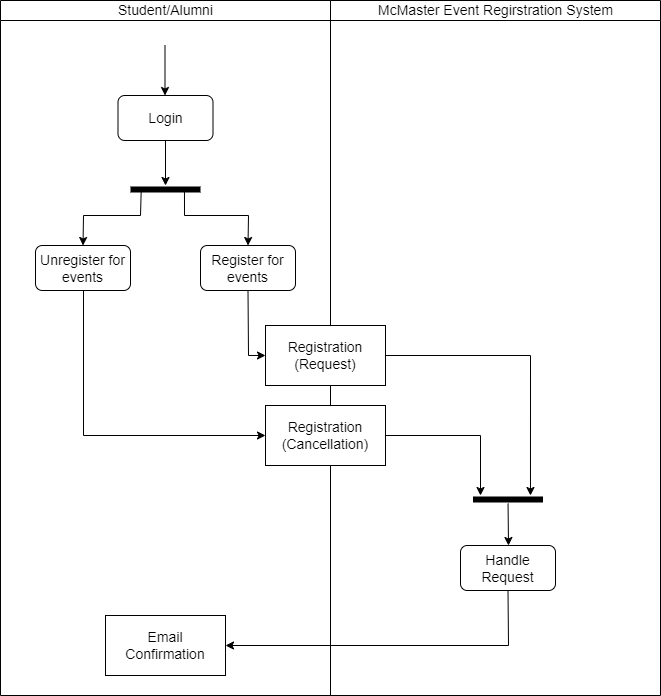
\includegraphics[scale=0.5]{Current_Situation.png}
\end{center}
\caption{Context Diagram}
\end{figure}

\subsection{The Context of the Work}

The context diagram depicted below illustrates the interactions of the system with adjacent external systems and services.
\begin{figure}[H]
\begin{center}
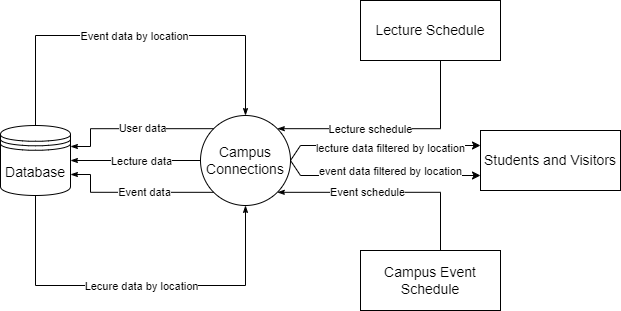
\includegraphics[scale=0.7]{Context_Diagram.png}
\end{center}
\caption{Current Event Registration Situation}
\end{figure}

\subsection{Work Partitioning}

\begin{table}[H]
  \begin{tabular}{p{0.33\textwidth} | p{0.33\textwidth} | p{0.33\textwidth}}
  \toprule
  \textbf{Event Name} & \textbf{Input/Output} & \textbf{Summary}\\
  \midrule
  Provide lecture schedule & IN: Lecture schedule & Give schedule of lectures when there is an update and after every semester\\
  \midrule
  Provide event schedule & IN: Event schedule & Give schedule of campus events periodically and when there is an update\\
  \midrule
  Record user data & OUT: User data & Record user related data, including user settings, user friends and registered events\\
  \midrule
  Record lecture data & OUT: Event data & Record lecture data, including lecture name,  time, duration and location\\
  \midrule
    Record event data & OUT: Event data & Record event data, including event name,  time,  duration and location\\
  \midrule
  Display event schedule & IN: event data, OUT: event data filtered by location & Display events that are going to be held in in a given building\\
  \midrule
  Display lecture schedule & IN: lecture data, OUT: lecture data filtered by location & Display lectures that are going to be held in in a given building\\
  \bottomrule
\end{tabular}
 \caption{Business Event List} 
 \label{TblEventList}
\end{table}

\subsection{Specifying a Business Use Case (BUC)}

The following is an activity diagram for the Display event schedule process. The trigger of this business user case will be user interaction, and input will be campus event data from database. What will be displayed is a schedule of events held inside a specific building with detailed event information.
\begin{figure}[H]
\begin{center}
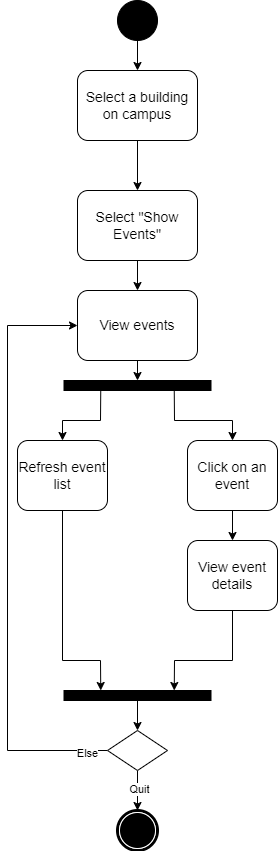
\includegraphics[scale=0.5]{BUC_Activity_Diagram.png}
\end{center}
\caption{Activity diagram for Display Event Schedule Process}
\end{figure}

\section{Business Data Model and Data Dictionary}
\subsection{Business Data Model}

The following UML class diagram shows all types of business data that will be used in this project.\\
All the classes represent corresponding business data, all these entries and their attributes will be defined and explained in the data dictionary.
class are defined in the data dictionary.
\begin{figure}[H]
\begin{center}
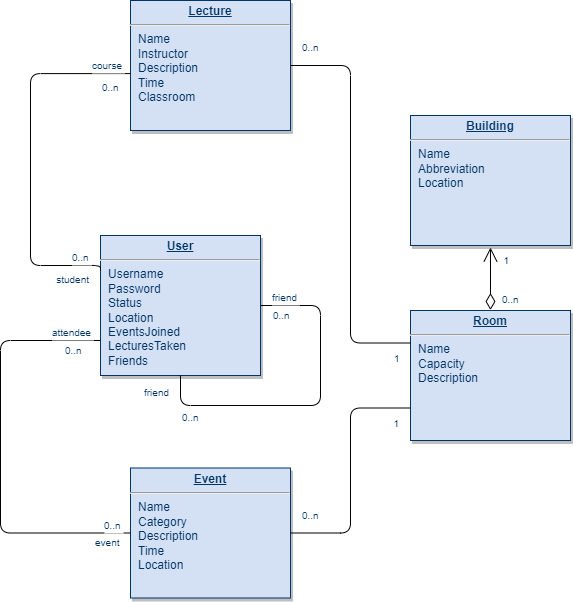
\includegraphics[scale=0.5]{Business_Data_Model.png}
\end{center}
\caption{UML class model}
\end{figure}

\subsection{Data Dictionary}
This section will include definition of all classes in UML class model and their attributes. Some self-explanatory attributes like name will be ignored.
\begin{longtable}
 {p{0.3\textwidth} | p{0.4\textwidth} | p{0.3\textwidth}}
  \toprule
  \textbf{Name} & \textbf{Content} & \textbf{Type}\\
  \midrule
  Lecture & McMaster course data & Class\\
  \midrule
  Lecture.Instructor & Course instructor & Attribute\\
  \midrule
  Lecture.Time & Course schedule & *HH/MM/SS
24 hour clock*\\
  \midrule
  Lecture.Classroom & Course location & Room\\
  \midrule
  Event & McMaster on-campus event data & Class\\
  \midrule
  Event.Category & Held by which department & Attribute\\
  \midrule
  Event.Time & Event time & *HH/MM/SS
24 hour clock*\\
  \midrule
  Lecture.Location & Event location & Room\\
  \midrule
  User & User account data, friends data, location,  event \& lecture attendance & Class\\
  \midrule
  User.Location & Geographic location & Attribute\\
  \midrule
  User.Status & Online or not & Boolean, Attribute\\
  \midrule
  User.EventsJoined & List of event & Event, Attribute\\
  \midrule
  User.LecturesTaken & List of lecture & Lecture, Attribute\\
  \midrule
  User.Friends & List of friends & User , Attribute\\
  \midrule
  Building & McMaster main campus building & Class\\
  \midrule
  Building.Abbreviation & Abbreviation of building name & Attribute\\
  \midrule
  Building.Location & Geographic location & Attribute\\
  \midrule
  Room & Room inside a building & Class\\
  \midrule
  Room.Capacity & Room capacity & Number, Attribute\\
  \bottomrule
  \caption{Data Dictionary} \label{TblDataDict}\\
\end{longtable}

\section{The Scope of the Product}
\subsection{Product Boundary}

The use case diagram depicted below identifies the boundaries between the users and the product.
\begin{figure}[H]
\begin{center}
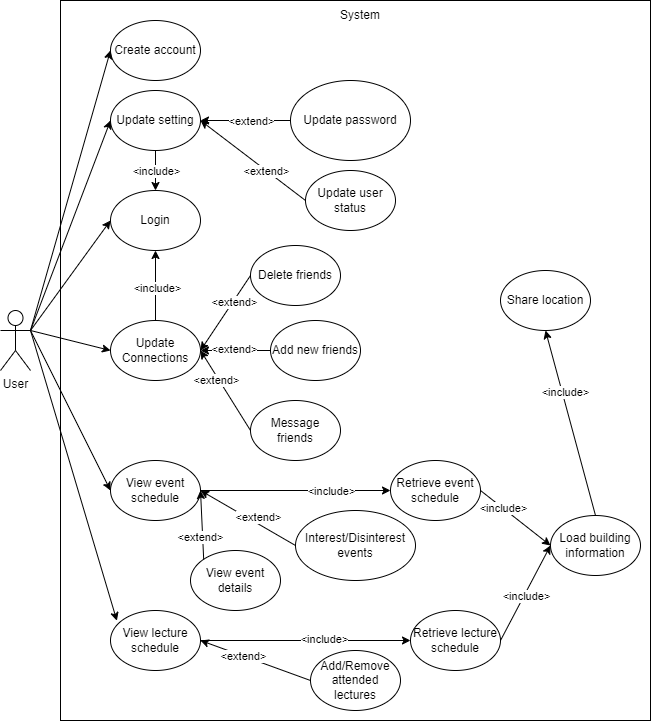
\includegraphics[scale=0.5]{Use_Case_Diagram.png}
\end{center}
\caption{Use Case Diagram}
\end{figure}

\subsection{Product Use Case Table}

\begin{longtable}
 {p{0.1\textwidth} | p{0.4\textwidth} | p{0.2\textwidth} | p{0.3\textwidth}}
  \toprule
  \textbf{PUC No} & \textbf{PUC Name} & \textbf{Actor/s} & \textbf{Input \& Output}\\
  \midrule
  1 & Create Account & User & Username \& Password (in)\\
  \midrule
  2 & Update Password & User & Username \& New Password (in)\\
  \midrule
  3 & Update User Status & User & New Status (in)\\
  \midrule
  4 & Login & User & Username \& Password (in),  Response message (out)\\
   \midrule
  5 & Add New Friend & User & Friend Username (in), Friend Request (out)\\
  \midrule
  6 & Delete Friend & User & Friend Username (in), Confirmation Message (out)\\
  \midrule
  7 & Message Friend & User & Message Content (in), Message Sent Notification (out)\\
  \midrule
  8 & View Event Details & User & User Interaction (in), Event details (out)\\
  \midrule
  9 & Interest/Disinterest Event & User & User Interaction \& Event Name (in)\\
  \midrule
  10 & Add/Remove attended lecture & User & User Interaction \& Lecture Name (in)\\
  \midrule
  11 & Retrieve Event Schedule & System & New Schedule (out)\\
  \midrule
  12 & Retrieve Lecture Schedule & System & New Schedule (out)\\
  \midrule
  13 & Load Building Information & System & Location \& Sensor data (in),  Building Name (out)\\
  \bottomrule
  \caption{Product Use Case} \label{TblPUC}\\
\end{longtable}

\subsection{Individual Product Use Cases (PUC's)}
\textbf{Use case \#1:} Create Account\\
\textbf{Precondition:} None\\
\textbf{Trigger:} The user clicks on create account button\\
\textbf{Outcome}
\begin{enumerate}
    \item User provides the required information
    \item System verifies all required information has been provided
    \item System securely registers user information
    \item User is redirected back to the Home page
\end{enumerate}
\textbf{Postcondition:} The user has successfully created an account and account information is stored and secured in a database.


\noindent\\
\textbf{Use case \#2:} Update Password\\
\textbf{Precondition:} The user has already created an account\\
\textbf{Trigger:} The user clicks on change password button\\
\textbf{Outcome}
\begin{enumerate}
	\item User navigates to change password page
    \item User provides old password
    \item User provides new password
    \item System verifies old password is correct and new password is valid
    \item System updates password of current user in the database
    \item User is redirected back to the Home page
\end{enumerate}
\textbf{Postcondition:} The user has successfully changed the password.


\noindent\\
\textbf{Use case \#3:} Update User Status\\
\textbf{Precondition:} The user has already created an account\\
\textbf{Trigger:} The user clicks on change status button\\
\textbf{Outcome}
\begin{enumerate}
	\item User navigates to change status page
    \item User updates status to a new status
    \item System updates user status and redirects back to the Home page
\end{enumerate}
\textbf{Postcondition:} The user status has been changed successfully.


\noindent\\
\textbf{Use case \#4:} Login\\
\textbf{Precondition:} The user has already created an account\\
\textbf{Trigger:} The user clicks on login button on the home page\\
\textbf{Outcome}
\begin{enumerate}
	\item User navigates to login page
    \item System verifies all required information has been provided and matches the database record
    \item User is redirected to the home page as alogged-in user
\end{enumerate}
\textbf{Postcondition:} The user has successfully logged in to the created account with all settings and connections loaded from the database.


\noindent\\
\textbf{Use case \#5:} Add New Friend\\
\textbf{Precondition:} The user has already logged in\\
\textbf{Trigger:} The user searches for another user and sends a friend request\\
\textbf{Outcome}
\begin{enumerate}
	\item User searches for another user
    \item User sends a friend request
    \item System sends the request and user information to the destined user
    \item Destined user accepts/rejects the request
    \item User receives a notification
\end{enumerate}
\textbf{Postcondition:} The user gets a new connection in their friends list.\\
\textbf{Postcondition 2:} The user is rejected and gets a notification about that.


\noindent\\
\textbf{Use case \#6:} Delete Friend\\
\textbf{Precondition:} The user has already logged in and has at lease one friend\\
\textbf{Trigger:} The user clicks delete button on friend page\\
\textbf{Outcome}
\begin{enumerate}
	\item User searches for a friend
    \item User deletes the friend
    \item System sends a confirmation prompt
    \item User continues to delete
    \item User receives a notification
\end{enumerate}
\textbf{Postcondition:} The friend is deleted from user's friends list.\\


\noindent\\
\textbf{Use case \#7:} Message Friend\\
\textbf{Precondition:} The user has already logged in and has at lease one friend\\
\textbf{Trigger:} The user texts a friend on friend page\\
\textbf{Outcome}
\begin{enumerate}
	\item User searches for a friend
    \item User start to text the friend
    \item System sends message to the destined friend
\end{enumerate}
\textbf{Postcondition:} The friend receives a message from the user.\\


\noindent\\
\textbf{Use case \#8:} View Event Details\\
\textbf{Precondition:} The user has already logged in and necessary sensors are working properly\\
\textbf{Trigger:} The user clicks on an event\\
\textbf{Outcome}
\begin{enumerate}
	\item User moves the device to target a building on campus
    \item User finds a list of events
    \item User clicks on one of the event
    \item System displays more information about the event
\end{enumerate}
\textbf{Postcondition:} The content, time and location of the event are displayed.\\


\noindent\\
\textbf{Use case \#9:} Interest/Disinterest Event\\
\textbf{Precondition:} The user has already logged in and had a target building\\
\textbf{Trigger:} The user clicks on interest/disinterest button\\
\textbf{Outcome}
\begin{enumerate}
	\item User browses the event list of the target
	\item User navigates to an event detail page with a specific name
	\item User clicks on the corresponding button
    \item System sends the request to the database
    \item System displays the new state of the event
\end{enumerate}
\textbf{Postcondition:} The user event list in the database is updated and the UI changes correspondingly.\\


\noindent\\
\textbf{Use case \#10:} Add/Remove Attended lecture\\
\textbf{Precondition:} The user has already logged in and had a target building\\
\textbf{Trigger:} The user clicks on add/remove button\\
\textbf{Outcome}
\begin{enumerate}
	\item User browses the lecture list of the target
	\item User navigates to a lecture detail page with a specific course code
	\item User clicks on the corresponding button
    \item System sends the request to the database
    \item System displays the new state of the lecture
\end{enumerate}
\textbf{Postcondition:} The user lecture list in the database is updated and the UI changes correspondingly.\\


\noindent\\
\textbf{Use case \#11:} Retrieve Event Schedule\\
\textbf{Precondition:} None\\
\textbf{Trigger:} A request to update schedule is sent or trigger by the system timer\\\
\textbf{Outcome}
\begin{enumerate}
	\item System sends a request to the on-campus schedule interface
    \item System gets the up-to-date schedule
    \item System stores the new schedule to the database
\end{enumerate}
\textbf{Postcondition:} The new schedule is stored in the database and will be utilized later.\\


\noindent\\
\textbf{Use case \#12:} Retrieve Lecture Schedule\\
\textbf{Precondition:} None\\
\textbf{Trigger:} A request to update schedule is sent or trigger by the system timer\\\
\textbf{Outcome}
\begin{enumerate}
	\item System sends a request to lecture schedule interface
    \item System gets the up-to-date schedule
    \item System stores the new schedule to the database
\end{enumerate}
\textbf{Postcondition:} The new schedule is stored in the database and will be utilized later.\\


\noindent\\
\textbf{Use case \#13:} Load Building Information\\
\textbf{Precondition:} Location share is allowed and sensors are set properly\\
\textbf{Trigger:} A request for event/lecture schedule is sent by the user\\
\textbf{Outcome}
\begin{enumerate}
	\item System gets geographic location and sensor data from the device
    \item System finds the most likely building on campus
    \item System displays building information
\end{enumerate}
\textbf{Postcondition:} The system provides information of the building the user locates now.\\
\section{Functional Requirements}
\subsection{Functional Requirements}
\begin{enumerate}
    \item The system shall allow users to create accounts.\\
        \textbf{Rationale:} Users must be associated with accounts to identify themselves and expand their social networking.\\
        \textbf{Fit Criterion:} Users must be able to create an account with a unique username and a password.\\
    \item The system shall allow users to change their password.\\
        \textbf{Rationale:} This will allow users to improve the security of their account and recover the account if they forget their password.\\
        \textbf{Fit Criterion:} Users may change password in the settings menu after proving their identity. The user must be notified afterwards.\\
    \item The system shall allow users to add friends.\\
        \textbf{Rationale:} One of the main purposes of this application is to make students connect with peers easily. For this to happen, they should be able to make friends on this social media platform.\\
        \textbf{Fit Criterion:} Users can search for other users through username and send a friend request, added friends can be removed from the friend list.\\
    \item The system shall allow users to delete friends.\\
        \textbf{Rationale:} When users add users as friends by accident or they no longer connect with each other, they should be able to remove them from the friend list.\\
        \textbf{Fit Criterion:} Users can remove any friends from their friend list.\\
    \item The system shall allow users to send text messages to other users.\\
        \textbf{Rationale:} This will make the app more interactive and encourage and enhance socialization between users.\\
        \textbf{Fit Criterion:} Users must be able send messages and to view received messages.\\
    \item The system shall allow users to share their location with others.\\
        \textbf{Rationale:} For the purpose of expanding social networking, users shall be able to share their current location with friends to meet in person.\\
        \textbf{Fit Criterion:} Users should be able to share their real-time location with friends as long as they agree on the corresponding terms.\\
    \item The system shall allow users to view events on the McMaster University campus.\\
        \textbf{Rationale:} Currently there is no way for students of McMaster University to keep up with all the different types of events that are hosted by different clubs and departments. This is one of the main purposes of this application to allow users to discover the time and place for as many events as possible in an intuitive manner\\
        \textbf{Fit Criterion:} Users will be able to see current / upcoming events at campus buildings that they are looking at / positioned near as well as a cumulative list of nearing events.\\
    \item The system shall allow users to pin events they are interested in.\\
        \textbf{Rationale:} It will be much easier for users to find events they are interested in and willing to join again. So that they do not have to browse the event list again and again. While their friends can see what events they are likely to join.\\
        \textbf{Fit Criterion:} Users should be able to pin an event from the event list, this event will be displayed on the user page and accessible to all their friends.\\
    \item The system shall allow users to unpin events.\\
        \textbf{Rationale:} In case users are no longer interested in the event or they pinned the event by mistake.\\
        \textbf{Fit Criterion:} Users shall be able to unpin an event they pinned before.\\
    \item The system shall allow users to view lecture schedule information.\\
        \textbf{Rationale:} This will allow users to verify their availability for events without needing to leave the app.\\
        \textbf{Fit Criterion:} Users must be able view lecture times and locations. \\
    \item The system shall allow users to pin lectures they are attending.\\
        \textbf{Rationale:} Sharing schedules with friends can increase friendship. If two friends are taking the same course, they can join lectures, discuss assignments and prepare for midterms together. So it is important for the system to have the functionality to display lectures a user is taking.\\
        \textbf{Fit Criterion:} Users should be able to pin a lecture from the list as attended lecture, this lecture will be displayed on the user page and accessible to all their friends.\\
    \item The system shall allow users to unpin lectures.\\
        \textbf{Rationale:} In case users are no longer taking the lecture or they added the lecture by mistake.\\
        \textbf{Fit Criterion:} Users shall be able to unpin a lecture they pinned before.\\
    \item The system shall have administrator accounts that have special modification access.\\
        \textbf{Rationale:} Administrator accounts should be utilized for the purpose of providing accurate and up-to-date event and lecture information.\\
        \textbf{Fit Criterion:} The system shall be able to mark specific users as administrators and give them access to edit, add and remove all in-app assets.\\
    \item The system shall allow users with an administrator account to add, edit, and remove events.\\
        \textbf{Rationale:} The event information must be up to date and accurate. The administrator account will maintain all events so that there is a singular source of information. Additionally, this reduces the chances of errors being introduced to the system.\\
        \textbf{Fit Criterion:} A new event can be created only by a user who is logged in as an administrator. The information for those events can be changed only by administrators. Events can be deleted only by administrators.\\
    \item The system shall allow users with an administrator account to add, edit, and remove lectures from the schedule.\\
        \textbf{Rationale:} The lecture information must be up to date and accurate as well. Administrators are needed to manage the schedule.\\
        \textbf{Fit Criterion:} A lecture on the schedule can be created, deleted, or updated by a user who logged in as an administrator.
    \item Each event shall be associated with a club/department, location and time.\\
        \textbf{Rationale:} In order for the application to schedule events for the users to see and interact with, all specific details about the event should be provided to the system\\
        \textbf{Fit Criterion:} When a department/club requests for an event to be posted on the application, they have to provide details about the building and room number it will be held in, along with the date and time the event will take place at.\\
    \item Each lecture shall be associated with an instructor, location and time.\\
        \textbf{Rationale:} In order to find empty rooms and help users who want to attend specific lectures, all details about the lectures should be provided to the system.\\
        \textbf{Fit Criterion:} When a lecture is added or modified, all the details mentioned above must be set as mandatory fields.\\
    \item The system shall allow users to create a virtual avatar.\\
        \textbf{Rationale:} A customizable avatar makes user accounts more personal and improves the immersiveness of the app. \\
        \textbf{Fit Criterion:} When the user creates an account, they will be prompted to design an avatar with some basic level of customization provided in the application. This avatar will be used to virtually identify the user.\\
    \item The system shall allow users to modify a virtual avatar.\\
        \textbf{Rationale:} The user might feel the need to update the appearance of their avatar to better represent themself. \\
        \textbf{Fit Criterion:} The avatar created in the user's registration process can be modified at any time through the settings menu.\\
    \item The system shall recognize buildings on campus.\\
        \textbf{Rationale:} When navigating the campus, users should be able to see their avatar on the map and recognize the buildings through their camera with some XR technologies.\\
        \textbf{Fit Criterion:} User must see their avatars moving correspondingly on the map when they travel on campus, and when they observe a specific building through their camera, the application should recognize it and display details about this building.\\
\end{enumerate}


\section{Look and Feel Requirements}
\subsection{Appearance Requirements}
\begin{itemize}
  \item The product shall have a user-friendly layout, with icons being intuitive and screen components not being congested.
  \item The product shall provide visual feedback to the users when they're using different features and switching pages.
  \item The product shall adapt to different mobile screen sizes.
\end{itemize}
\subsection{Style Requirements}
\begin{itemize}
  \item The colors and themes shall be consistent across different pages.
  \item The color scheme used shall be appealing and not cause eye strain.
\end{itemize}
\lips

\section{Usability and Humanity Requirements}
\subsection{Ease of Use Requirements}
\begin{itemize}
  \item The product shall have a UI that is clear and easy to navigate.
\end{itemize}
\subsection{Personalization and Internationalization Requirements}
\begin{itemize}
  \item The product shall provide information about ongoing lectures and events personalized to each user.
  \item The product shall allow users to customize their profiles and avatars.
\end{itemize}
\subsection{Learning Requirements}
\begin{itemize}
  \item The product shall include a short tutorial on its features on the first launch, and be available upon request from the user.
  \item The product shall be designed so that it is easy for users to remember how to use its features after learning them once.
\end{itemize}

  \subsection{Understandability and Politeness Requirements}
\begin{itemize}
  \item The product shall have a simple and intuitive design that is easy for users to understand.
  \item The product shall abstain from using technical and software-specific language.
\end{itemize}
\subsection{Accessibility Requirements}
\begin{itemize}
  \item The colors used by the different components of the product shall contrast enough for items on the screen to be more easily visible.
\end{itemize}

\section{Performance Requirements}
\subsection{Speed and Latency Requirements}
\lips
\subsection{Safety-Critical Requirements}
\lips
\subsection{Precision or Accuracy Requirements}
\lips
\subsection{Robustness or Fault-Tolerance Requirements}
\lips
\subsection{Capacity Requirements}
\lips
\subsection{Scalability or Extensibility Requirements}
\lips
\subsection{Longevity Requirements}
\lips

\section{Operational and Environmental Requirements}
\subsection{Expected Physical Environment}
\begin{itemize}
  \item The product will be installed on the user's smartphone (iPhone or Android).
  \item The product will be used around the main campus of McMaster University.
\end{itemize}

\subsection{Wider Environment Requirements}
\begin{itemize}
  \item N/A
\end{itemize}

\subsection{Requirements for Interfacing with Adjacent Systems}
\begin{itemize}
  \item The product shall interface with the latest four major releases of iOS.
  \item The product shall interface with the latest four major releases of Android OS.
  \item The product shall interface with ARKit for AR capabilities on Apple devices.
  \item The product shall interface with ARCore for AR capabilities on Android devices.
\end{itemize}

\subsection{Productization Requirements}
\begin{itemize}
  \item The product shall be downloadable through the App Store for Apple devices.
  \begin{itemize}
    \item \textbf{Fit criterion:} The product can be downloaded onto an Apple device through the App Store.
  \end{itemize}
  \item The product shall be downloadable through the Google Play Store for Android devices.
  \begin{itemize}
    \item \textbf{Fit criterion:} The product can be downloaded onto an Android device through the Google Play Store.
  \end{itemize}
\end{itemize}

\subsection{Release Requirements}
\begin{itemize}
  \item N/A
\end{itemize}

\section{Maintainability and Support Requirements}
\subsection{Maintenance Requirements}

\qquad Major updates could be rolled out during periods of reduced usage such as Reading Week, after exams, or Spring semester.
This will allow significant time to stablize the update and test them before the updates are applied to the users.

Additionally, the administrator can perfrom maintenance on the database and server to check the correct operation of the product.
This will maximize the availability of the product.

\subsection{Supportability Requirements}

\qquad Feature requests or issues can be sent to the product GitHub.
These opened issues will be discussed by the maintainers and communicated through the issue on how they will be dealt with.

A user manual will be complied and stored in the GitHub, this manual will be updated with Frequently Asked Questions and other entries as additional features are introduced.
The application will direct users to this manual in the menu.

\subsection{Adaptability Requirements}

\qquad Currently, Android 11 and above are recieving security updates, and therefore this product will be accessible in Android 11 and above.

This product will be accessible in Windows 10 and above, as these have not reached end of life and recieving security updates.

This product will be accesible in iOS 15 and above, as these are still currently recieving security support.

This product may be ported to other universities in Ontario, Canada, or other countries.
Although the product is designed to work for university, this can be porte to other large events and buildings to help users navigate and coordinate better.

\section{Security Requirements}
\subsection{Access Requirements}

There will be three levels of access. 

The first will be before login and account creation, where anyone can access. They must not have access to anything beyond the login, account creation, and account recovery pages.

The second will be after login that verifies their identity, where the user has provided information matching the McMaster student or faculty member with McMaster email account. Only the user can access this page.

The third level will the the administrator account, used for adding, deleting, or editing official events. This account can be accessed by login that verifies that they are the maintainer, this will be used by the maintainers to check the functionality of the product  and pull logs that are not accessible to users.

\subsection{Integrity Requirements}

The product will prevent introduction of duplicate data, to guarantee that all user identities are unique.

In the future, the database and server can protect itself from excessive use with a load balancer and additional servers being added.

\subsection{Privacy Requirements}

All data collected must be encrypted on disk in the server by standard encryption algorithm.
All data collected must be encrypted on transit by industry standard encryption algorithm.

The product will require users to agree on the terms prior to account creation and additional data submission.
The product must erase all data if the user requests, or when account is deleted.
Additionally, accounts that are inactive for a certain period of time will have their account deleted after notice to prevent unnecessary data being held.

\subsection{Audit Requirements}

N/A (This currently does not apply, once the product is ready to be used in multiple universities and regions, audit requirements will be reconsidered.)

\subsection{Immunity Requirements}

The product must only use open source libraries with many users and continuous security updates. 
As open source libraries are used by millions of people, vulnerabilities are found and patched much earlier.

The product must undergo vulnerability checks before a build is pushed to the users.
This will prevent vulnerabilities from inadequate codes from being introduced to user devices.

Security updates must be done as soon as possible when they are announced for used packages.
This will reduce the chances of novel attacks from affecting the product.

\section{Cultural Requirements}
\subsection{Cultural Requirements}
\begin{itemize}
  \item The product shall not be offensive to any marginalized groups.
  \begin{itemize}
    \item \textbf{Fit Criterion:} The product shall not use any language or symbols deemed offensive by a marginalized group.
  \end{itemize}
  \item The product shall not be offensive to any religious or groups.
  \begin{itemize}
    \item \textbf{Fit Criterion:} The product shall not use any language or symbols deemed offensive by a religious or ethnic group.
  \end{itemize}
\end{itemize}

\section{Compliance Requirements}
\subsection{Legal Requirements}

\qquad The data collected from users will be handled as per the same legal requirements for the university.
As this application will be used in university, it is subject to the same regulations that the university is beholden to.
In the future, different functions can be developed to match specific university or state/country requirements, but this is currently not in scope.

\subsection{Standards Compliance Requirements}

\qquad The encryption on data in storage and in transit must be industry standard.
This ensures that the application is safe and can be scaled and expanded to other universities or interested parties when needed.

\qquad The application will abide by the guidelines set by the university and club managers, adding options to accomodate their requests.
This will prevent the application from compromising the security standards of the university.

\section{Open Issues}
\begin{itemize}
  \item To target iOS devices, a device capable of building iOS apps is required.
\end{itemize}

\section{Off-the-Shelf Solutions}
\subsection{Ready-Made Products}
\begin{itemize}
  \item \textbf{Snapchat:} Snapchat is an existing social media platform that makes use of AR technology through its Lenses feature which provides various filters and effects that users can apply to their content.
  \item \textbf{Instagram:} Instagram is another platform that incorporates AR in the form of filters and effects.
  \item \textbf{TikTok:} TikTok similarly uses AR for visual effects and filters.
  \item \textbf{Facebook:} Many clubs at McMaster use Facebook Groups to coordinate events.
  \item \textbf{Meetup:} Meetup is another platform designed for organizing and finding events and other social gatherings.
  \item \textbf{CampusGroups:} CampusGroups is a platform that focuses specifically on university student groups. It allows universities to create private communities for various events and other student engagement activities.
\end{itemize}
\subsection{Reusable Components}
% This is outlining features of existing apps that could be "reused" by our app, verify this is appropriate for this section
\begin{itemize}
  \item Event planning, scheduling and searching
  \item Friends and Groups system
  \item AR-integrated content (virtual billboards, avatars, \dots)
  \item Asynchrnous communication (text messages, voice messages)
\end{itemize}
\subsection{Products That Can Be Copied}
% TODO: Look further into this for open-source or otherwise free products that could be legally "copied"
N/A
\section{New Problems}
\subsection{Effects on the Current Environment}

This application will not take place of any existing official tools. It intends to improve certain social networking processes students are following and provide a platform for users to connect with each other better. The following are some changes that will impact users.\\
\noindent\\
\textbf{Expand Networking}\\
Students will be able to expand networking when attending events lectures on this social media platform. Users may lose connection with peers when there is a failure in the system. 
\noindent\\
\textbf{Event Registration}\\
Students and alumni will be able to login with their McMaster email and write comments about on campus events, which means there will be a risk of personal identification information (PII) leakage if the data is not stored securely.
\noindent\\
\textbf{Available Room Management}\\
This application can be utilized to get information about lecture time and location which should not be displayed publicly. Therefore insecure data storage may lead to data breaches.

\subsection{Effects on the Installed Systems}

The application will be completely stand alone and will not be interfacing with any existing systems.  As described in the previous section, this application should not affect or replace any existing systems.

\subsection{Potential User Problems}

Any potential adverse reactions related to using the device in which application is being launched on (mobile device or tablet) would extend to the use of this application.  Any adverse reactions of Virtual Reality and Augment Reality, like nausea, dizziness and disorientation would be introduced to the use of the application as well.

\subsection{Limitations in the Anticipated Implementation Environment That May
Inhibit the New Product}

\begin{itemize}
\item The database free plan is not able to cope with our projected user growth pattern.
\item Low quality internet connection will lead to latency between user inputs and in-game reactions or even failures of loading in-game assets.
\item The accuracy of input data totally depends on device sensor. Low accuracy data may cause bad user experience.
\end{itemize}

\subsection{Follow-Up Problems}

Any failures or downtime on Unity game engine and its third-party libraries may affect the availability of this application. In-game schedules may fail to load when the event and lecture schedule interfaces are down or the two external systems are under maintenance. There will also be a risk of violating privacy laws in the future since the application is collection personal information and there may be new laws prohibit this kind of information collection.

\section{Tasks}
\subsection{Project Planning}

The project schedule will follow the deadline for the deliverables outlined in the SFWRENG
4G06 course outline.

\begin{table}[H]
    \centering
    \begin{tabular}{|p{0.2\linewidth} | p{0.5\linewidth}| p{0.3\linewidth} |}
    \hline
    \textbf{Phase} & \textbf{Task} & \textbf{Deadline}\\
    \hline
    Revision 0 & Hazard Analysis & Oct 20, 2023 \\
     \cline{2-3} & Verification and Validation Plan & Nov 3, 2023 \\
     \cline{2-3} & Proof of Concept Demo & Nov 13-24, 2023\\
     \cline{2-3} & Design Document & Jan 17, 2024\\
     \cline{2-3} & Demonstration & Feb 5-16, 2024\\
     \cline{2-3} & Verification and Validation Report & Mar 6, 2024\\
     \hline
     Revision 1 & Final Demonstration & Mar 18-29, 2024\\
     \cline{2-3} & EXPO Demonstration & April 2024\\
     \cline{2-3} & Final Documentation & Apr 4, 2024\\
     
     
     
     
     
    \hline
    \end{tabular}
    \caption{Project Plan}
    \label{TblProjectTasks}
\end{table}

\subsection{Planning of the Development Phases}
The development of the project will be divided into two phases
\begin{itemize}
    \item Revision 0, initial development
    \item Revision 1, refinement of the project and documents
\end{itemize}
Revision 0 starts now and ends with the Verification and Validation Report. In this phase, the team will work on some design-related documents and specify the scope of the project, what skills the team will be using, and how the interaction of different components be. Then the team will start implementation as proof of concept and demonstrate their product to stakeholders. After that, the team will write a V\&V report based on the demonstration and stakeholder feedback.\\
Revision 1 will focus on the refinement of the application and documents. In the previous phase, the team finished a bunch of drafted documents, and in this phase, the team should put all effort into incorporating feedback into these documents and the application itself. There will not be any major new features added in Revision 1.

\section{Migration to the New Product}
\subsection{Requirements for Migration to the New Product}

\qquad There are no requirements to migrate to this product besides recruiting sufficient number of users.
With the the starting users, there may not be enough engagement for this application to be widely used.

\subsection{Data That Has to be Modified or Translated for the New System}

\qquad Currently, all data we need are in OSCARplus and club management part of the university administration.
These data will be requested via API or a new web based or internal input system will be made to move all the data over to our product.

As this product handles real time data, there is no need to migrate outdated data to the product.

\section{Costs}
\lips
\section{User Documentation and Training}
\subsection{User Documentation Requirements}
\lips
\subsection{Training Requirements}
\lips

\section{Waiting Room}
N/A

\section{Ideas for Solution}
Implementation ideas for solutions
\begin{itemize}
\item AR feature
	\begin{itemize}
	\item Vuforia supports some AR functionalities and works as a library of Unity
	\item gather.town might be a good design approach to follow after from the campus navigation and interaction perspective
	\end{itemize}
\item Server
	\begin{itemize}
	\item AWS might be a purchasable and reliable option for the back-end
	\end{itemize}
\end{itemize}

\newpage{}
\section*{Appendix --- Reflection}

The information in this section will be used to evaluate the team members on the
graduate attribute of Lifelong Learning.  Please answer the following questions:

\begin{enumerate}
  \item What knowledge and skills will the team collectively need to acquire to
  successfully complete this capstone project?  Examples of possible knowledge
  to acquire include domain specific knowledge from the domain of your
  application, or software engineering knowledge, mechatronics knowledge or
  computer science knowledge.  Skills may be related to technology, or writing,
  or presentation, or team management, etc.  You should look to identify at
  least one item for each team member.
  
  
\quad The team members will need to collectively acquire some technical and non-technical skills and knowledge in order to succeed in this capstone project. The following is a list of skills that are critical to the project and course deliverables.
  \begin{enumerate}[1]
      \item Presentation skills for demonstrations and capstone EXPO
      \item Documentation skills
      \item Team management skills including time management and work distribution
      \item Skills of Unity game development
      \item Skills of Unity AR development
      \item Integrating external backend systems into a Unity project
      \item Skills of git
      \item Front-end development skills
      \item Back-end development skills including server deployment and database
      \item Organizational skills to lead meetings and discussions on unclear topics in the project
  \end{enumerate}
  
  \item For each of the knowledge areas and skills identified in the previous
  question, what are at least two approaches to acquiring the knowledge or
  mastering the skill?  Of the identified approaches, which will each team
  member pursue, and why did they make this choice?
  
  
\quad For non-technical skills, team members can develop those skills by practicing and attending courses/workshops. Members can leverage LinkedIn Learning and McMaster workshops to develop management and organizational skills. For documentation and presentation skills, team members can also join related events hosted by the university or refer to past documents and presentations.\\
  There are even more resources available for developing technical skills. Online learning platforms like Udemy will be used for the team to learn new technology-specific domain knowledge and skills. Other online resources like YouTube tutorials and official documentation can help the team master those technical skills as well.\\
  Listed below under each team member’s name is a list of skills that the team member will focus on and why they decide to work on them.\\
    \begin{itemize}
      \item \textbf{Zihao Du}
      \begin{itemize}
          \item Skills: 1, 2, 3, 4, 8
      \end{itemize}
      Soft skills are quite important for a team and an engineer. And that's why I'd like to focus on soft skills like presentation skills and documentation skills. It will be not only critical to succeed in this capstone project but also beneficial to software engineering careers. Communication plays a very important role in software engineer's daily work and I will take this opportunity to further improve my skills.\\
      I'll also focus on Unity game development and front-end development because that attracts me the most and what I have the most experience in and I'd like to strengthen my skills and learn more about game development during this project.
  \end{itemize}
\end{enumerate}

\end{document}